\documentclass[10pt,a4paper]{article}

\usepackage[margin=0.75cm]{geometry}
\usepackage[utf8]{inputenc}

\usepackage{amsmath}
\usepackage{amssymb}
\usepackage{biblatex}
\usepackage{textcomp}
\usepackage{gensymb}
\usepackage{paracol}
\usepackage{parskip}
\usepackage{tikz}
\usepackage{titlesec}
\usepackage{verbatim}
\usepackage{xcolor}

\titleformat{\section}[block]{\Large\bfseries\filcenter\color{black}}{\thesection}{1em}{}
\titleformat{\subsection}[block]{\bfseries\filcenter\color{black}}{\thesubsection}{1em}{}

\setlength{\columnsep}{25pt}

\tikzset{
    rounded-box/.style = {draw=violet, fill=white, thin, rectangle, rounded corners, inner sep=5pt, inner ysep=10pt},
    rounded-box-title/.style = {fill=violet, text=white, font=\bfseries},
}

\addbibresource{references.bib}

\begin{document}
\title{Complex Variables}

\section{Complex Numbers}

\begin{paracol}{2}

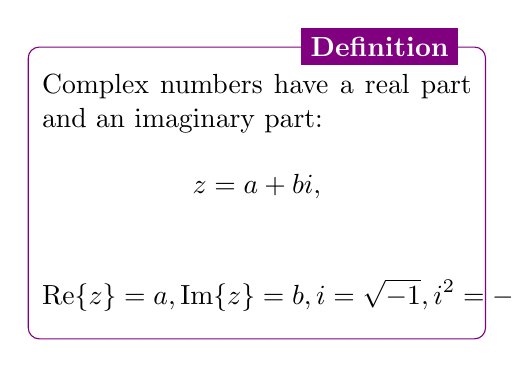
\begin{tikzpicture}
\node [rounded-box] (box){\begin{minipage}{0.45\textwidth}
    Complex numbers have a real part and an imaginary part:

    $$z = a + bi,$$

    $$\text{Re}\{z\} = a, \text{Im}\{z\} = b, i = \sqrt{-1}, i^2 = -1$$
\end{minipage}};
\node[rounded-box-title, left=10pt] at (box.north east) {Definition};
\end{tikzpicture}

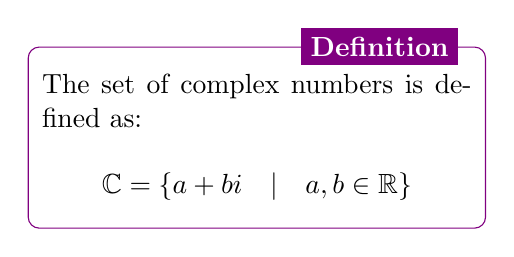
\begin{tikzpicture}
\node [rounded-box] (box){\begin{minipage}{0.45\textwidth}
    The set of complex numbers is defined as:

    $$\mathbb{C} = \{ a + bi \quad | \quad a, b \in \mathbb{R} \}$$
\end{minipage}};
\node[rounded-box-title, left=10pt] at (box.north east) {Definition};
\end{tikzpicture}

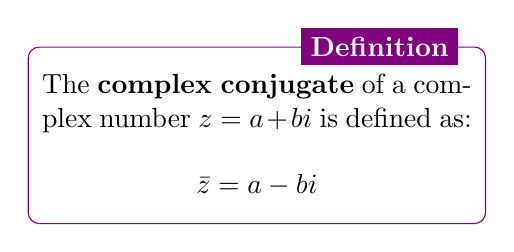
\begin{tikzpicture}
\node [rounded-box] (box){\begin{minipage}{0.45\textwidth}
    The \textbf{complex conjugate} of a complex number $z = a + bi$ is defined as:

    $$\bar{z} = a - bi$$
\end{minipage}};
\node[rounded-box-title, left=10pt] at (box.north east) {Definition};
\end{tikzpicture}

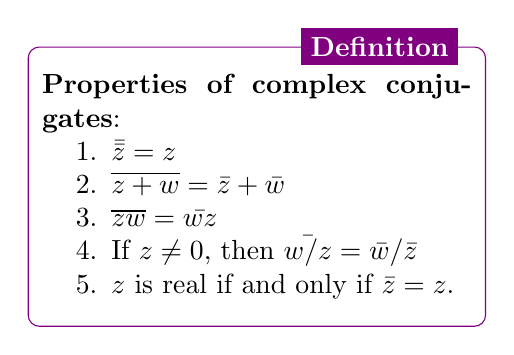
\begin{tikzpicture}
\node [rounded-box] (box){\begin{minipage}{0.45\textwidth}
    \textbf{Properties of complex conjugates}:

    \begin{enumerate}
        \item $\bar{\bar{z}} = z$
        \item $\overline{z + w} = \bar{z} + \bar{w}$
        \item $\overline{zw} = \bar{wz}$
        \item If $z \neq 0$, then $\bar{w / z} = \bar{w} / \bar{z}$
        \item $z$ is real if and only if $\bar{z} = z$.
    \end{enumerate}
\end{minipage}};
\node[rounded-box-title, left=10pt] at (box.north east) {Definition};
\end{tikzpicture}

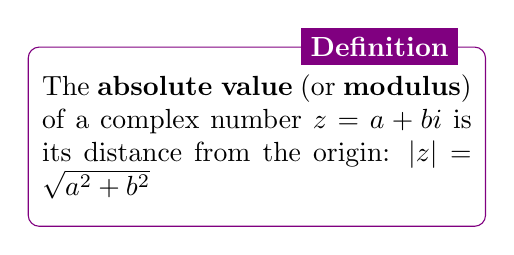
\begin{tikzpicture}
\node [rounded-box] (box){\begin{minipage}{0.45\textwidth}
    The \textbf{absolute value} (or \textbf{modulus}) of a complex number $z = a + bi$ is its distance from the origin: $|z| = \sqrt{a^2 + b^2}$
\end{minipage}};
\node[rounded-box-title, left=10pt] at (box.north east) {Definition};
\end{tikzpicture}

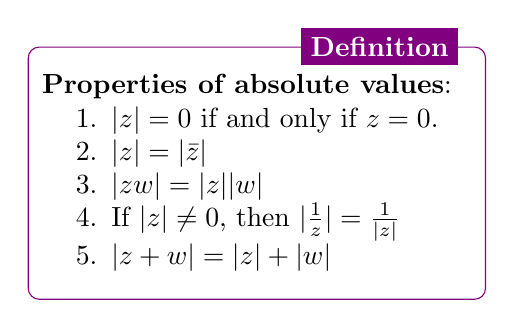
\begin{tikzpicture}
\node [rounded-box] (box){\begin{minipage}{0.45\textwidth}
    \textbf{Properties of absolute values}:

    \begin{enumerate}
        \item $|z| = 0$ if and only if $z = 0$.
        \item $|z| = |\bar{z}|$
        \item $|zw| = |z| |w|$
        \item If $|z| \neq 0$, then $|\frac{1}{z}| = \frac{1}{|z|}$
        \item $|z + w| = |z| + |w|$
    \end{enumerate}
\end{minipage}};
\node[rounded-box-title, left=10pt] at (box.north east) {Definition};
\end{tikzpicture}

\switchcolumn

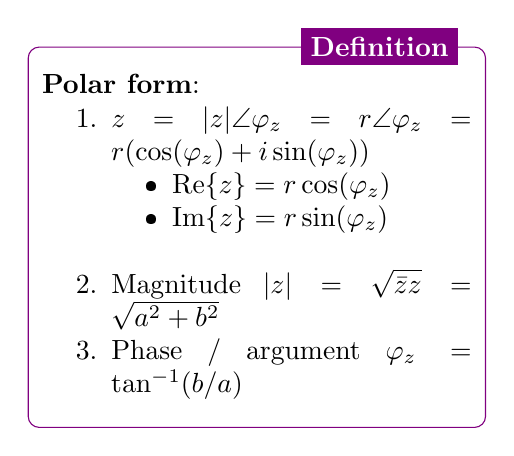
\begin{tikzpicture}
\node [rounded-box] (box){\begin{minipage}{0.45\textwidth}
    \textbf{Polar form}:

    \begin{enumerate}
        \item $z = |z| \angle \varphi_z = r \angle \varphi_z = r (\cos(\varphi_z) + i \sin(\varphi_z))$
        \begin{itemize}
            \item $\text{Re}\{z\} = r \cos(\varphi_z)$
            \item $\text{Im}\{z\} = r \sin(\varphi_z)$ \\
        \end{itemize}
        \item Magnitude $|z| = \sqrt{\bar{z}z} = \sqrt{a^2 + b^2}$
        \item Phase / argument $\varphi_z = \tan^{-1}(b/a)$
    \end{enumerate}
\end{minipage}};
\node[rounded-box-title, left=10pt] at (box.north east) {Definition};
\end{tikzpicture}

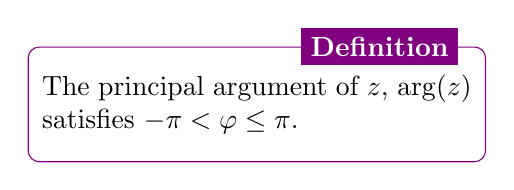
\begin{tikzpicture}
\node [rounded-box] (box){\begin{minipage}{0.45\textwidth}
    The principal argument of $z$, $\arg(z)$ satisfies $- \pi < \varphi \leq \pi$.
\end{minipage}};
\node[rounded-box-title, left=10pt] at (box.north east) {Definition};
\end{tikzpicture}

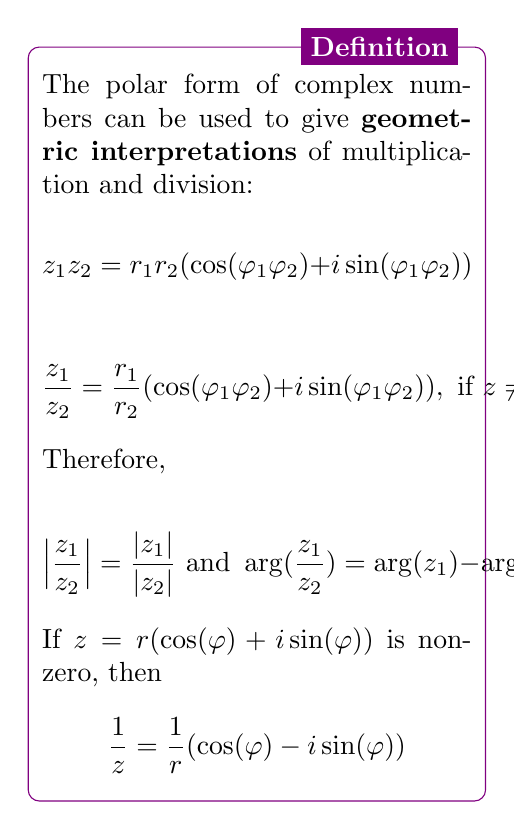
\begin{tikzpicture}
\node [rounded-box] (box){\begin{minipage}{0.45\textwidth}
    The polar form of complex numbers can be used to give \textbf{geometric interpretations} of multiplication and division:

    \vspace{-5pt}

    $$z_1 z_2 = r_1 r_2 ( \cos(\varphi_1 \varphi_2) + i \sin(\varphi_1 \varphi_2) )$$

    $$\frac{z_1}{z_2} = \frac{r_1}{r_2} ( \cos(\varphi_1 \varphi_2) + i \sin(\varphi_1 \varphi_2) ), \text{ if } z \neq 0$$

    Therefore,

    $$\Big| \frac{z_1}{z_2} \Big| = \frac{|z_1|}{|z_2|} \text{ and } \arg(\frac{z_1}{z_2}) = \arg(z_1) - \arg(z_2)$$

    If $z = r ( \cos(\varphi) + i \sin(\varphi))$ is non-zero, then

    $$\frac{1}{z} = \frac{1}{r} ( \cos(\varphi) - i \sin(\varphi) )$$
\end{minipage}};
\node[rounded-box-title, left=10pt] at (box.north east) {Definition};
\end{tikzpicture}

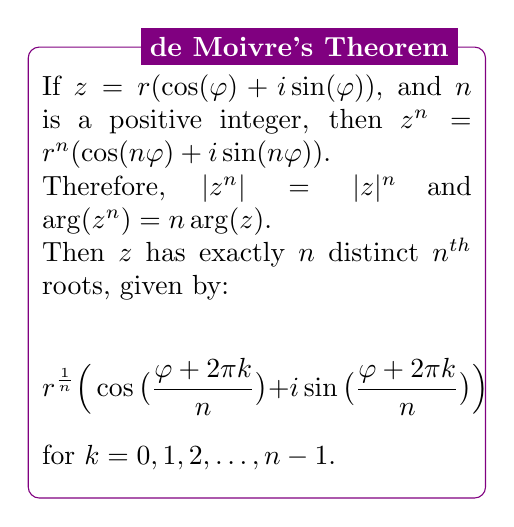
\begin{tikzpicture}
\node [rounded-box] (box){\begin{minipage}{0.45\textwidth}
    If $z = r ( \cos(\varphi) + i \sin(\varphi) )$, and $n$ is a positive integer, then $z^n = r^n ( \cos(n \varphi) + i \sin(n \varphi) )$.
    
    Therefore, $| z^n | = |z|^n$ and $\arg(z^n) = n \arg(z)$.

    Then $z$ has exactly $n$ distinct $n^{th}$ roots, given by:

    $$r^\frac{1}{n} \Big( \cos \big( \frac{\varphi + 2 \pi k}{n} \big) + i \sin \big( \frac{\varphi + 2 \pi k}{n} \big) \Big)$$

    for $k = 0, 1, 2, \dots, n - 1$.
\end{minipage}};
\node[rounded-box-title, left=10pt] at (box.north east) {de Moivre's Theorem};
\end{tikzpicture}

\end{paracol}

de Moivre's Formula, $e^{i \theta} \cdot \dots \cdot e^{i \theta} = e^{i (\theta + \dots + \theta)} = (e^{i \theta})^n = e^{i \cdot n \theta}$ can be used to derive equations for the sine and cosine:

$$
(\cos{\theta} + i \sin{\theta})^n = \cos{n \theta} + i \sin{n \theta}
$$

\textbf{Example}:

$\cos{2 \theta} + i \sin{2 \theta} = (\cos{\theta} + i \sin{\theta})^2 = \cos^2{\theta} + 2 i \sin{\theta} \cos{\theta} + (-1) \sin^2{\theta} = (\cos^2{\theta} - \sin^2{\theta}) + 2 i \sin{\theta} \cos{\theta}$

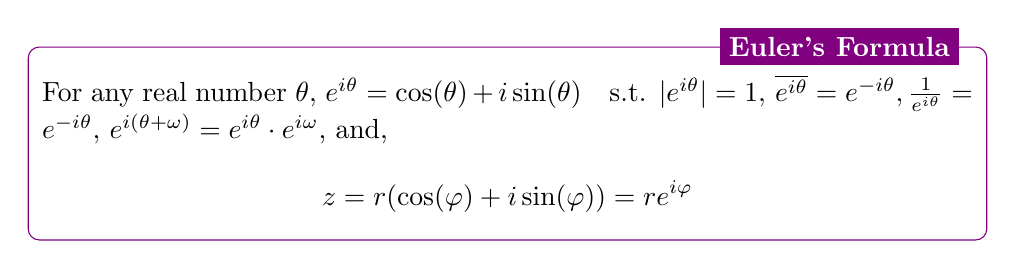
\begin{tikzpicture}
\node [rounded-box] (box){\begin{minipage}{0.975\textwidth}
    For any real number $\theta$, $e^{i \theta} = \cos(\theta) + i \sin(\theta) \quad \text{s.t. } | e^{i \theta} | = 1, \, \overline{e^{i \theta}} = e^{-i \theta}, \frac{1}{e^{i \theta}} = e^{- i \theta}, \, e^{i (\theta + \omega)} = e^{i \theta} \cdot e^{i \omega}$, and,

    $$z = r (\cos(\varphi) + i \sin(\varphi)) = r e^{i \varphi}$$
\end{minipage}};
\node[rounded-box-title, left=10pt] at (box.north east) {Euler's Formula};
\end{tikzpicture}

\textbf{Proof}: The exponential form of a complex number can be determined from a Taylor series:

$$
    e^{i \varphi} = 1 + (i \varphi) + \frac{(i \varphi)^2}{2!} + \frac{(i \varphi)^3}{3!} + \dots = \Big( 1 - \frac{\varphi^2}{2!} + \frac{\varphi^4}{4!} - \dots \Big) + i \Big( \varphi - \frac{\varphi^3}{3!} + \frac{\varphi^5}{5!} + \dots \Big) = \cos(\varphi) + i \sin(\varphi)
$$


\begin{tikzpicture}
\node [rounded-box] (box){\begin{minipage}{0.975\textwidth}
    $$e^{i \varphi} + 1 = 0$$
\end{minipage}};
\node[rounded-box-title, left=10pt] at (box.north east) {Euler's Identity};
\end{tikzpicture}
 \newpage
\section{Polynomials}

\begin{paracol}{2}

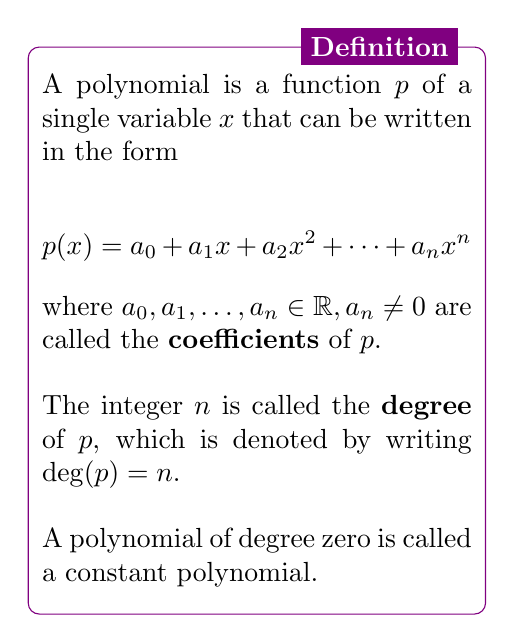
\begin{tikzpicture}
\node [rounded-box] (box){\begin{minipage}{0.45\textwidth}
    A polynomial is a function $p$ of a single variable $x$ that can be written in the form

    $$p(x) = a_0 + a_1 x + a_2 x^2 + \dots + a_n x^n$$

    where $a_0, a_1, \dots, a_n \in \mathbb{R}, a_n \neq 0$ are called the \textbf{coefficients} of $p$. \\

    The integer $n$ is called the \textbf{degree} of $p$, which is denoted by writing $\deg(p) = n$. \\
    
    A polynomial of degree zero is called a constant polynomial.
\end{minipage}};
\node[rounded-box-title, left=10pt] at (box.north east) {Definition};
\end{tikzpicture}

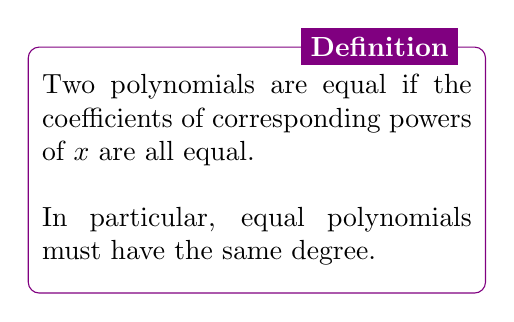
\begin{tikzpicture}
\node [rounded-box] (box){\begin{minipage}{0.45\textwidth}
    Two polynomials are equal if the coefficients of corresponding powers of $x$ are all equal. \\
    
    In particular, equal polynomials must have the same degree.
\end{minipage}};
\node[rounded-box-title, left=10pt] at (box.north east) {Definition};
\end{tikzpicture}

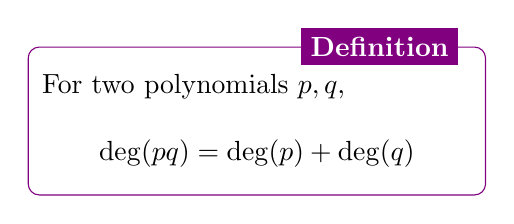
\begin{tikzpicture}
\node [rounded-box] (box){\begin{minipage}{0.45\textwidth}
    For two polynomials $p, q$,

    $$\deg(pq) = \deg(p) + \deg(q)$$
\end{minipage}};
\node[rounded-box-title, left=10pt] at (box.north east) {Definition};
\end{tikzpicture}

\switchcolumn

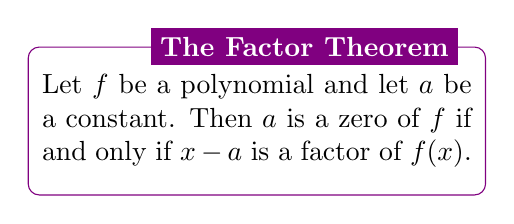
\begin{tikzpicture}
\node [rounded-box] (box){\begin{minipage}{0.45\textwidth}
    Let $f$ be a polynomial and let $a$ be a constant. Then $a$ is a zero of $f$ if and only if $x - a$ is a factor of $f(x)$.
\end{minipage}};
\node[rounded-box-title, left=10pt] at (box.north east) {The Factor Theorem};
\end{tikzpicture}

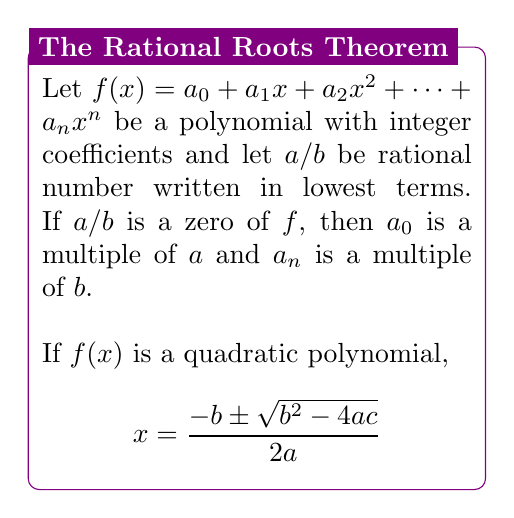
\begin{tikzpicture}
\node [rounded-box] (box){\begin{minipage}{0.45\textwidth}
    Let $f(x) = a_0 + a_1 x + a_2 x^2 + \dots + a_n x^n$ be a polynomial with integer coefficients and let $a / b$ be rational number written in lowest terms. If $a / b$ is a zero of $f$, then $a_0$ is a multiple of $a$ and $a_n$ is a multiple of $b$. \\

    If $f(x)$ is a quadratic polynomial,

    $$x = \frac{-b \pm \sqrt{b^2 - 4ac}}{2a}$$
\end{minipage}};
\node[rounded-box-title, left=10pt] at (box.north east) {The Rational Roots Theorem};
\end{tikzpicture}

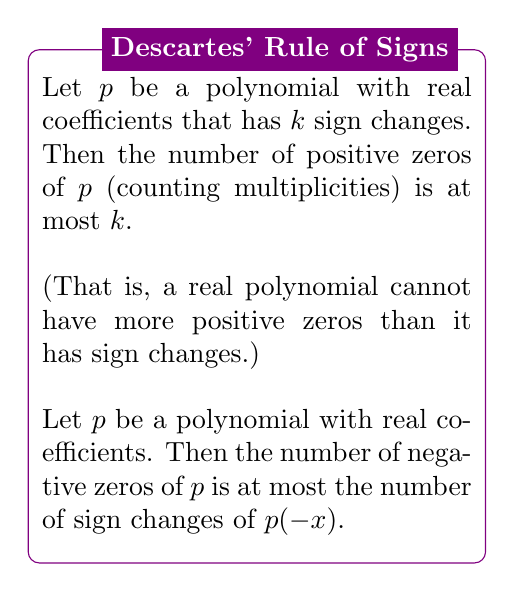
\begin{tikzpicture}
\node [rounded-box] (box){\begin{minipage}{0.45\textwidth}
    Let $p$ be a polynomial with real coefficients that has $k$ sign changes. Then the number of positive zeros of $p$ (counting multiplicities) is at most $k$. \\

    (That is, a real polynomial cannot have more positive zeros than it has sign changes.) \\

    Let $p$ be a polynomial with real coefficients. Then the number of negative zeros of $p$ is at most the number of sign changes of $p(-x)$.
\end{minipage}};
\node[rounded-box-title, left=10pt] at (box.north east) {Descartes' Rule of Signs};
\end{tikzpicture}

\end{paracol}

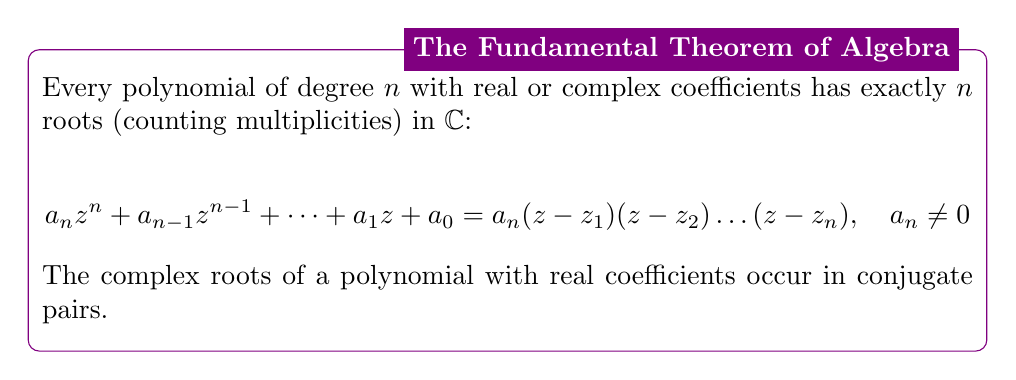
\begin{tikzpicture}
\node [rounded-box] (box){\begin{minipage}{0.975\textwidth}
    Every polynomial of degree $n$ with real or complex coefficients has exactly $n$ roots (counting multiplicities) in $\mathbb{C}$:

    $$
    a_n z^n + a_{n-1} z^{n-1} + \dots + a_1 z + a_0 = a_n (z - z_1) (z - z_2) \dots (z - z_n), \quad a_n \neq 0
    $$

    The complex roots of a polynomial with real coefficients occur in conjugate pairs.
\end{minipage}};
\node[rounded-box-title, left=10pt] at (box.north east) {The Fundamental Theorem of Algebra};
\end{tikzpicture}

\textbf{Example}: Consider the polynomial $p(x) = x^2 + 1$ in $\mathbb{R}$. It has no real roots. But in $\mathbb{C}$ it can be factored: $z^2 + 1 = (z + i) (z - i)$


\begin{tikzpicture}
\node [rounded-box] (box){\begin{minipage}{0.975\textwidth}
    The $n^\text{th}$ roots of $1$ are called the $n^\text{th}$ \textbf{roots of unity}.
\end{minipage}};
\node[rounded-box-title, left=10pt] at (box.north east) {Definition};
\end{tikzpicture}

\textbf{Example}: Since $1 = 1 e^{i \cdot 0}$, $1^{1/n} = \sqrt[n]{1} \cdot e^{i (\frac{0}{n} + \frac{2k \pi}{n})}, \, k = 0, 1, \dots, n - 1 = e^{i (\frac{2k \pi}{n})}, \, k = 0, 1, \dots, n - 1$
 \newpage
% \section{Topology in the Complex Plane}

\begin{paracol}{2}

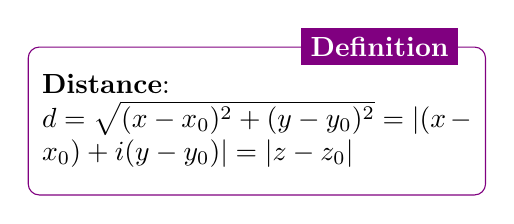
\begin{tikzpicture}
\node [rounded-box] (box){\begin{minipage}{0.45\textwidth}
    \textbf{Distance}:
    
    $d = \sqrt{(x - x_0)^2 + (y - y_0)^2} = | (x - x_0) + i (y - y_0) | = | z - z_0 |$
\end{minipage}};
\node[rounded-box-title, left=10pt] at (box.north east) {Definition};
\end{tikzpicture}

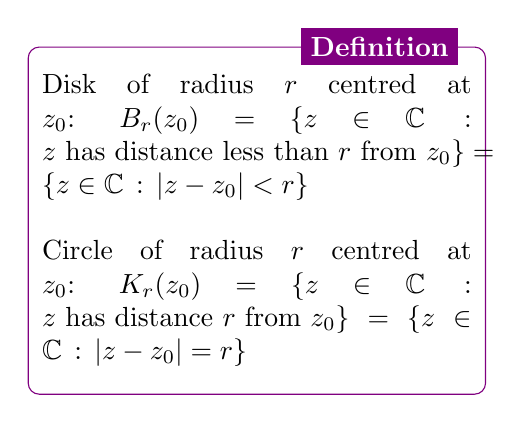
\begin{tikzpicture}
\node [rounded-box] (box){\begin{minipage}{0.45\textwidth}
    Disk of radius $r$ centred at $z_0$: $B_r(z_0) = \{ z \in \mathbb{C} \, : \, z \text{ has distance less than } r \text{ from } z_0 \} = \{ z \in \mathbb{C} \, : \, | z - z_0 | < r \}$ \\

    Circle of radius $r$ centred at $z_0$: $K_r(z_0) = \{ z \in \mathbb{C} \, : \, z \text{ has distance } r \text{ from } z_0 \} = \{ z \in \mathbb{C} \, : \, | z - z_0 | = r \}$
\end{minipage}};
\node[rounded-box-title, left=10pt] at (box.north east) {Definition};
\end{tikzpicture}

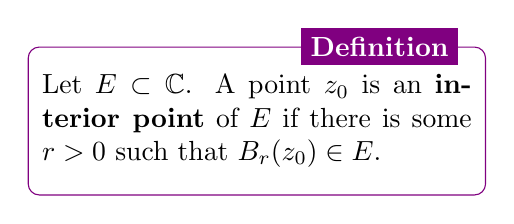
\begin{tikzpicture}
\node [rounded-box] (box){\begin{minipage}{0.45\textwidth}
    Let $E \subset \mathbb{C}$. A point $z_0$ is an \textbf{interior point} of $E$ if there is some $r > 0$ such that $B_r(z_0) \in E$.
\end{minipage}};
\node[rounded-box-title, left=10pt] at (box.north east) {Definition};
\end{tikzpicture}

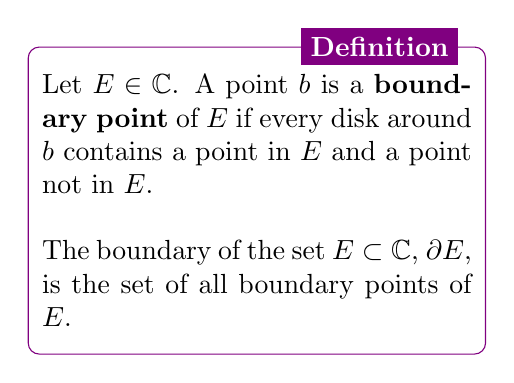
\begin{tikzpicture}
\node [rounded-box] (box){\begin{minipage}{0.45\textwidth}
    Let $E \in \mathbb{C}$. A point $b$ is a \textbf{boundary point} of $E$ if every disk around $b$ contains a point in $E$ and a point not in $E$. \\

    The boundary of the set $E \subset \mathbb{C}$, $\partial E$, is the set of all boundary points of $E$.
\end{minipage}};
\node[rounded-box-title, left=10pt] at (box.north east) {Definition};
\end{tikzpicture}

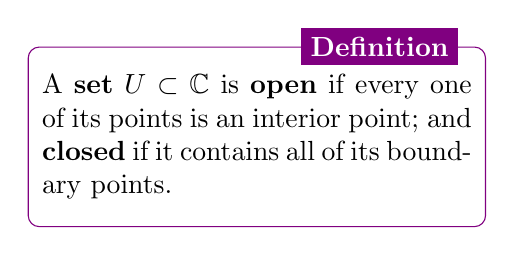
\begin{tikzpicture}
\node [rounded-box] (box){\begin{minipage}{0.45\textwidth}
    A \textbf{set} $U \subset \mathbb{C}$ is \textbf{open} if every one of its points is an interior point; and \textbf{closed} if it contains all of its boundary points.
\end{minipage}};
\node[rounded-box-title, left=10pt] at (box.north east) {Definition};
\end{tikzpicture}

\textbf{Examples}:

\begin{itemize}
    \item $\{ z \in \mathbb{C} \, : \, | z - z_0 | < r \}$ and $\{ z \in \mathbb{C} \, : \, | z - z_0 | > r \}$ are open.

    \item $\mathbb{C}$ and $\empty$ are open.

    \item $\{ z \in \mathbb{C} \, : \, | z - z_0 | \leq r \}$ and $\{ z \in \mathbb{C} \, : \, | z - z_0 | = r \}$ are closed.

    \item $\mathbb{C}$ and $\empty$ are closed.

    \item $\{ z \in \mathbb{C} \, : \, | z - z_0 | < r \} \cup \{ z \in \mathbb{C} \, : \, | z - z_0 | = r \text{ and Im}(z - z_0) > 0 \}$ is neither open nor closed.
\end{itemize}

\switchcolumn

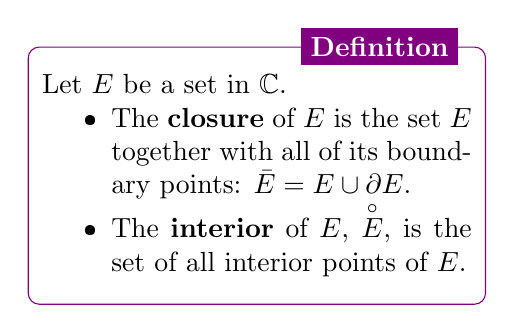
\begin{tikzpicture}
\node [rounded-box] (box){\begin{minipage}{0.45\textwidth}
    Let $E$ be a set in $\mathbb{C}$.

    \begin{itemize}
        \item The \textbf{closure} of $E$ is the set $E$ together with all of its boundary points: $\bar{E} = E \cup \partial E$.

        \item The \textbf{interior} of $E$, $\overset{\circ}{E}$, is the set of all interior points of $E$.
    \end{itemize}
\end{minipage}};
\node[rounded-box-title, left=10pt] at (box.north east) {Definition};
\end{tikzpicture}

\textbf{Examples}:

\begin{itemize}
    \item $\overline{B_r(z_0)} = B_r(z_0) \cup K_r(z_0) = \{ z \in \mathbb{C} \, : \, | z - z_0 | \leq r$.

    \item $\overline{K_r(z_0)} = K_r(z_0)$.

    \item $\overline{B_r(z_0) \backslash \{ z_0 \}} = \{ z \in \mathbb{C} \, : \, | z - z_0 | \leq r \}$.

    \item With $E = \{ z \in \mathbb{C} \, : \, | z - z_0 | \leq r \}$, $\overset{\circ}{E} = B_r(z_0)$.

    \item With $E = K_r(z_0)$, $\overset{\circ}{E} = \empty$.
\end{itemize}

A set is connected if it is "in one piece".

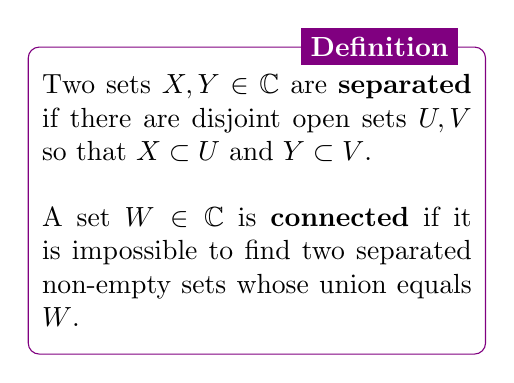
\begin{tikzpicture}
\node [rounded-box] (box){\begin{minipage}{0.45\textwidth}
    Two sets $X, Y \in \mathbb{C}$ are \textbf{separated} if there are disjoint open sets $U, V$ so that $X \subset U$ and $Y \subset V$. \\
    
    A set $W \in \mathbb{C}$ is \textbf{connected} if it is impossible to find two separated non-empty sets whose union equals $W$.
\end{minipage}};
\node[rounded-box-title, left=10pt] at (box.north east) {Definition};
\end{tikzpicture}

\textbf{Example}: $X = [0, 1), Y = (1, 2]$ are separated: For example, choose $U = B_1(0)$ and $V = B_1(2)$. Thus, $X \cup Y = [0, 2] \backslash \{ 1 \}$ is not connected. It is hard to check whether a set is connected!

For open sets, there is a much easier-to-check criterion:

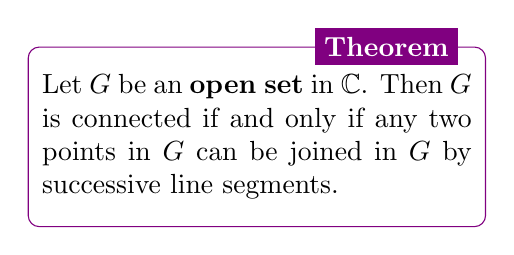
\begin{tikzpicture}
\node [rounded-box] (box){\begin{minipage}{0.45\textwidth}
    Let $G$ be an \textbf{open set} in $\mathbb{C}$. Then $G$ is connected if and only if any two points in $G$ can be joined in $G$ by successive line segments.
\end{minipage}};
\node[rounded-box-title, left=10pt] at (box.north east) {Theorem};
\end{tikzpicture}

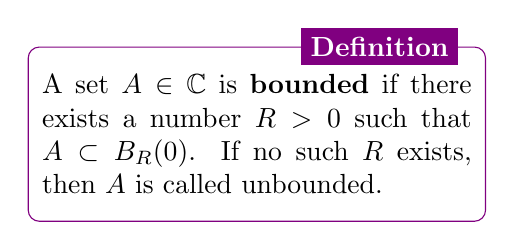
\begin{tikzpicture}
\node [rounded-box] (box){\begin{minipage}{0.45\textwidth}
    A set $A \in \mathbb{C}$ is \textbf{bounded} if there exists a number $R > 0$ such that $A \subset B_R(0)$. If no such $R$ exists, then $A$ is called unbounded.
\end{minipage}};
\node[rounded-box-title, left=10pt] at (box.north east) {Definition};
\end{tikzpicture}

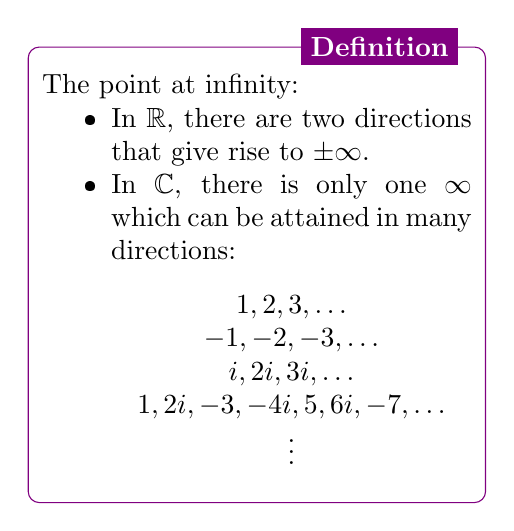
\begin{tikzpicture}
\node [rounded-box] (box){\begin{minipage}{0.45\textwidth}
    The point at infinity:

    \begin{itemize}
        \item In $\mathbb{R}$, there are two directions that give rise to $\pm \infty$.

        \item In $\mathbb{C}$, there is only one $\infty$ which can be attained in many directions: $$\begin{array}{c}
            1, 2, 3, \dots \\
            -1, -2, -3, \dots \\
            i, 2i, 3i, \dots \\
            1, 2i, -3, -4i, 5, 6i, -7, \dots \\
            \vdots
        \end{array}$$
    \end{itemize}
\end{minipage}};
\node[rounded-box-title, left=10pt] at (box.north east) {Definition};
\end{tikzpicture}

\end{paracol}
 \newpage
% \section{Complex Functions and Iteration}

\subsection{Subsection}

\begin{paracol}{2}

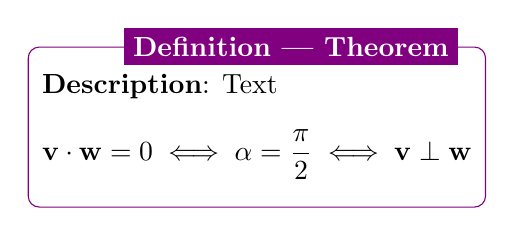
\begin{tikzpicture}
\node [rounded-box] (box){\begin{minipage}{0.45\textwidth}
    \textbf{Description}: Text
    $$\mathbf{v} \cdot \mathbf{w} = 0 \iff \alpha = \frac{\pi}{2} \iff \mathbf{v} \perp \mathbf{w}$$
\end{minipage}};
\node[rounded-box-title, left=10pt] at (box.north east) {Definition | Theorem};
\end{tikzpicture}

\end{paracol}
 \newpage
% \section{Analytic Functions}

\subsection{Subsection}

\begin{paracol}{2}

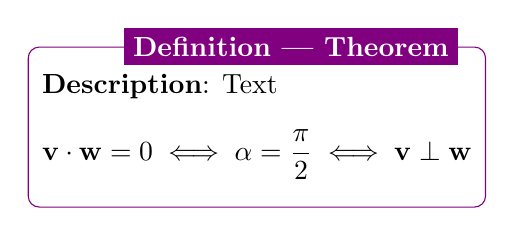
\begin{tikzpicture}
\node [rounded-box] (box){\begin{minipage}{0.45\textwidth}
    \textbf{Description}: Text
    $$\mathbf{v} \cdot \mathbf{w} = 0 \iff \alpha = \frac{\pi}{2} \iff \mathbf{v} \perp \mathbf{w}$$
\end{minipage}};
\node[rounded-box-title, left=10pt] at (box.north east) {Definition | Theorem};
\end{tikzpicture}

\end{paracol}
 \newpage
% \section{Conformal Mappings}

\subsection{Subsection}

\begin{paracol}{2}

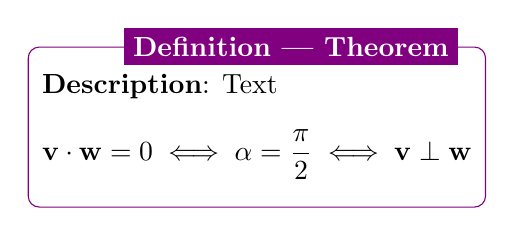
\begin{tikzpicture}
\node [rounded-box] (box){\begin{minipage}{0.45\textwidth}
    \textbf{Description}: Text
    $$\mathbf{v} \cdot \mathbf{w} = 0 \iff \alpha = \frac{\pi}{2} \iff \mathbf{v} \perp \mathbf{w}$$
\end{minipage}};
\node[rounded-box-title, left=10pt] at (box.north east) {Definition | Theorem};
\end{tikzpicture}

\end{paracol}
 \newpage
% \section{Complex Integration}

\subsection{Subsection}

\begin{paracol}{2}

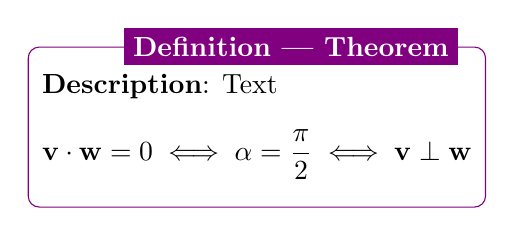
\begin{tikzpicture}
\node [rounded-box] (box){\begin{minipage}{0.45\textwidth}
    \textbf{Description}: Text
    $$\mathbf{v} \cdot \mathbf{w} = 0 \iff \alpha = \frac{\pi}{2} \iff \mathbf{v} \perp \mathbf{w}$$
\end{minipage}};
\node[rounded-box-title, left=10pt] at (box.north east) {Definition | Theorem};
\end{tikzpicture}

\end{paracol}
 \newpage
% \section{Power Series}

\subsection{Subsection}

\begin{paracol}{2}

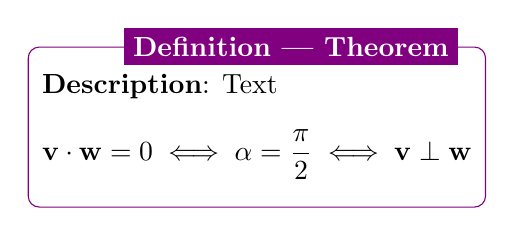
\begin{tikzpicture}
\node [rounded-box] (box){\begin{minipage}{0.45\textwidth}
    \textbf{Description}: Text
    $$\mathbf{v} \cdot \mathbf{w} = 0 \iff \alpha = \frac{\pi}{2} \iff \mathbf{v} \perp \mathbf{w}$$
\end{minipage}};
\node[rounded-box-title, left=10pt] at (box.north east) {Definition | Theorem};
\end{tikzpicture}

\end{paracol}
 \newpage
% \section{Laurent Series and the Residue Theorem}

\subsection{Subsection}

\begin{paracol}{2}

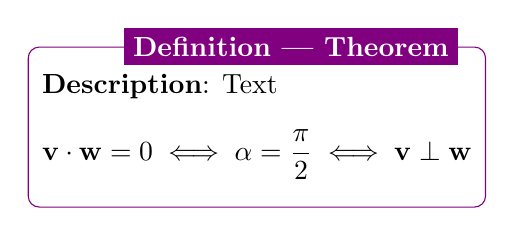
\begin{tikzpicture}
\node [rounded-box] (box){\begin{minipage}{0.45\textwidth}
    \textbf{Description}: Text
    $$\mathbf{v} \cdot \mathbf{w} = 0 \iff \alpha = \frac{\pi}{2} \iff \mathbf{v} \perp \mathbf{w}$$
\end{minipage}};
\node[rounded-box-title, left=10pt] at (box.north east) {Definition | Theorem};
\end{tikzpicture}

\end{paracol}
 \newpage

\nocite{*}
\printbibliography

\end{document}
